\documentclass[tikz,border=5pt]{standalone}
\usetikzlibrary{arrows.meta,positioning,shapes.geometric}
\begin{document}
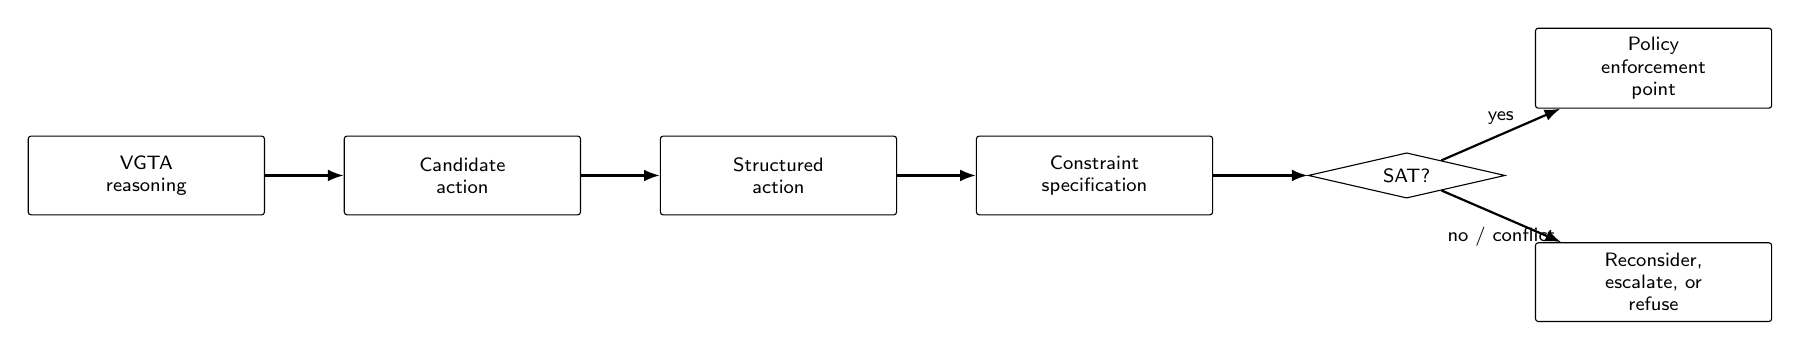
\begin{tikzpicture}[
  box/.style={draw, rounded corners=1pt, minimum width=30mm, minimum height=10mm, align=center, font=\sffamily\scriptsize},
  decision/.style={draw, diamond, aspect=2, minimum width=25mm, align=center, font=\sffamily\scriptsize, inner sep=1pt},
  arrow/.style={-{Latex[length=2mm]}, thick}
]
\node[box] (reason) {VGTA\\reasoning};
\node[box, right=of reason] (cand) {Candidate\\action};
\node[box, right=of cand] (repr) {Structured\\action};
\node[box, right=of repr] (csl) {Constraint\\specification};
\node[decision, right=12mm of csl] (smt) {SAT?};
\node[box, above right=7mm and 10mm of smt] (permit) {Policy\\enforcement\\point};
\node[box, below right=7mm and 10mm of smt] (reject) {Reconsider,\\escalate, or\\refuse};
\draw[arrow] (reason) -- (cand);
\draw[arrow] (cand) -- (repr);
\draw[arrow] (repr) -- (csl);
\draw[arrow] (csl) -- (smt);
\draw[arrow] (smt) -- node[above, font=\sffamily\scriptsize]{yes} (permit);
\draw[arrow] (smt) -- node[below, font=\sffamily\scriptsize]{no / conflict} (reject);
\end{tikzpicture}
\end{document}
